\documentclass[sigplan,10pt]{acmart}

\usepackage{tikz}

\setcopyright{rightsretained}
\copyrightyear{2020}
\acmYear{2020}
\acmDOI{}
\acmConference[]{}{}{}
\acmBooktitle{}
\acmPrice{}
\acmISBN{}

\hyphenation{da-ta-cen-ter da-ta-cen-ters time-stamp time-stamps time-stamped hard-links}

\begin{document}
\title{Reordering Elements in List CRDTs}

\author{Martin Kleppmann}
\email{mk428@cl.cam.ac.uk}
\orcid{0000-0001-7252-6958}
\affiliation{%
  \institution{Department of Computer Science and Technology}
  \streetaddress{15 JJ Thomson Avenue}
  \city{Cambridge}
  \state{}
  \postcode{CB3 0FD}
  \country{United Kingdom}
}

\begin{abstract}
\end{abstract}

\settopmatter{printfolios=true} % Recommended EuroSys formatting
\maketitle

\section{Introduction}

Conflict-free Replicated Data Types (CRDTs) allow multiple replicas to concurrently modify some shared data object, while ensuring that all replicas eventually converge towards the same, consistent state~\cite{Shapiro:2011un}.
CRDT algorithms have been developed for various different datatypes, and one of the most important datatypes is the \emph{list} (also called \emph{sequence} or \emph{array} datatype).
A list is a collection of elements in a total order, which is chosen by the user.

Replicated lists can be used to implement a variety of important applications, such as:
\begin{itemize}
    \item text editors (text is a list of characters);
    \item graphics applications (a list of graphical objects, where the order determines visibility: objects ``further down'' may be occluded or filtered by the objects ``higher up'', as illustrated in Fig.~\ref{fig:smiley});
    \item to-do lists and task trackers (a list of tasks, where the order may reflect the relative priority of tasks as chosen by the user).
\end{itemize}

\begin{figure*}
  \centering
  \includegraphics{smiley.pdf}
  \caption{Graphics software often places objects in a list that determines the z-index; objects higher in the list occlude lower ones. %
    Here, the eyeballs are placed above the yellow face, and the pupils in turn are placed above the eyeballs.}
  \label{fig:smiley}
\end{figure*}

Many list CRDTs have been developed, such as WOOT~\cite{Oster:2006wj}, Treedoc~\cite{Preguica:2009fz}, RGA~\cite{Roh:2011dw}, Causal Trees/Timestamped Insertion Trees~\cite{Grishchenko:2014eh,Attiya:2016kh}, Logoot \cite{Weiss:2009ht,Weiss:2010hx}, and LSEQ \cite{Nedelec:2013ky,Nedelec:2016eo}.
Moreover, most of the field of Operational Transformation algorithms is dedicated to algorithms for collaboratively editable text, i.e.\ lists~\cite{Ellis:1989ue,Nichols:1995fd,Ressel:1996wx,Sun:1998vf,Oster:2006tr}.

All of the aforementioned algorithms allow replicas to \emph{insert} or \emph{delete} elements anywhere in the list.
However, none of them have explicit support for \emph{reordering} or \emph{moving} elements from one position to another position in the list.
This is a surprising omission because reordering is a commonly required operation: in many to-do list applications, a user can drag and drop list elements to reorder them, and graphics software allows users to reorder the object list with commands such as ``bring to front'' (which moves an object to the top of the list) and ``send to back'' (which moves an object to the bottom).

In this paper we introduce an algorithm that allows an existing list CRDT to be extended with a reorder operation.
The algorithm is generic in the sense that it can be implemented on top of any of the aforementioned list CRDTs.

\section{A Generic Reordering Algorithm}

\begin{acks}
Martin Kleppmann is supported by a Leverhulme Trust Early Career Fellowship and by the Isaac Newton Trust.
\end{acks}

\bibliographystyle{ACM-Reference-Format}
\bibliography{references}{}
\end{document}
